\documentclass{article}

% CS224W project proposal (Project type 1: real-world application of GNNs).
% Dataset statistics are reproduced by analysis/iapd_careers.py.
\usepackage[preprint,nonatbib]{neurips_2022}
\usepackage[numbers,sort&compress]{natbib}

\usepackage[utf8]{inputenc}
\usepackage[T1]{fontenc}
\usepackage{hyperref}
\usepackage{url}
\usepackage{booktabs}
\usepackage{float}
\usepackage{amsmath,amsfonts,amssymb}
\usepackage{microtype}
\usepackage{xcolor}
\usepackage{tikz}
\usetikzlibrary{positioning,arrows.meta}
\usepackage[colorinlistoftodos,textsize=scriptsize]{todonotes}
\makeatletter\renewcommand{\@noticestring}{}\makeatother

\title{Who Moves Next? Predicting Financial-Adviser Job Moves with Heterogeneous GNNs}

\author{%
  Nino Triandafilidis\\
  Stanford University\\
  \texttt{ninot@stanford.edu}
}

\begin{document}

\maketitle

\noindent\textbf{Group members:} Nino Triandafilidis

% ---------------------------------------------------------------------------
\section{Application domain and dataset}

\textbf{Domain.} Recruiting rests on a chain of decisions: finding candidates, deciding whom to contact first, matching them to roles and judging fit. We tackle one subproblem of sourcing: predicting which professionals are likely to change employers soon, so that recruiters and sourcing platforms can contact them first, while they are open to a move, instead of cold-calling everyone.

\textbf{Dataset.} We use the SEC's Investment Adviser Public Disclosure (IAPD) registry~\citep{sec_iapd}, which lists every registered US investment adviser representative with named employers and firm IDs, registration start and end dates to the day, and branch office addresses. Each daily file holds only current registrants, so we rebuild careers from 14 copies of the registry (June 2016 -- October 2026): the current SEC file plus 13 archived copies from the Internet Archive~\citep{wayback}. Joining them gives about 600K advisers, 49.5K firms, 1.34M employment periods and 475K firm changes. The dataset is \emph{public}: the raw files are public records, and the processed tables and code are at \url{https://github.com/nino-triandafilidis/cs224w-project/tree/main/dataset/iapd}.

\textbf{Task.} On a cut-off date, for every registered adviser, predict whether they move to a different firm within the next 12 months, using only what was known on that date. Firm changes caused by mergers or rebrands (many advisers switching between the same two firms at once) and people who leave the industry are excluded. We use several cut-off dates and split them by time into training, validation and test.

\textbf{Metric.} Only 4--5\% of advisers move in a year, so we report the hit rate among the top 1\% of advisers ranked by the model (how many of the people a recruiter would call actually move) and PR-AUC, always next to the base rate.

\textbf{Why this dataset.} It is the only public source we found with real, dated career moves between named employers at scale. Recruiting datasets with candidate histories are private or carry synthetic or LLM-generated fields. It also defines colleagues exactly: advisers at the same firm and branch at the same time.

% ---------------------------------------------------------------------------
\section{Graph ML techniques}

\begin{figure}[H]
  \centering
  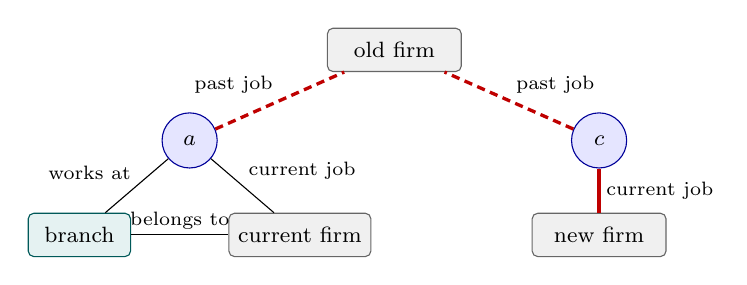
\begin{tikzpicture}[
      font=\footnotesize,
      adv/.style={circle, draw=blue!60!black, fill=blue!10, minimum size=7mm, inner sep=0pt},
      firm/.style={rounded corners=2pt, draw=black!60, fill=black!6, minimum width=17mm, minimum height=5.5mm},
      br/.style={rounded corners=2pt, draw=teal!70!black, fill=teal!10, minimum width=13mm, minimum height=5.5mm},
      past/.style={dash pattern=on 3pt off 2pt},
      hl/.style={draw=red!75!black, line width=1.2pt},
      lab/.style={font=\scriptsize, inner sep=2pt}]
    \node[adv] (a) at (-2.6,0) {$a$};
    \node[adv] (c) at (2.6,0) {$c$};
    \node[firm] (fold) at (0,1.15) {old firm};
    \node[firm] (fnew) at (2.6,-1.2) {new firm};
    \node[firm] (fcur) at (-1.2,-1.2) {current firm};
    \node[br] (b) at (-4.0,-1.2) {branch};
    \draw (a) -- node[lab, above right] {current job} (fcur);
    \draw (a) -- node[lab, above left] {works at} (b);
    \draw (b) -- node[lab, above] {belongs to} (fcur);
    \draw[hl, past] (a) -- node[lab, above left] {past job} (fold);
    \draw[hl, past] (c) -- node[lab, above right] {past job} (fold);
    \draw[hl] (c) -- node[lab, right] {current job} (fnew);
  \end{tikzpicture}
  \caption{Graph schema at a cut-off date, built only from earlier records. Dashed edges are dated past jobs. Red: a two-hop path from adviser $a$ through an old firm to a former colleague $c$ who has already moved, a pattern hand-built features capture poorly.}
  \label{fig:schema}
\end{figure}

\textbf{Graph.} Nodes are advisers, firms and branches (firm plus postcode). Edges are current jobs, past jobs with start and end dates, ``works at'' between advisers and branches, and ``belongs to'' between branches and firms. Past-job edges connect each adviser to former colleagues (Fig.~\ref{fig:schema}). Adviser features are tenure at the current firm, career length, and the number of past firms and moves; firm and branch features are size and change in headcount over the past year.

\textbf{Model.} Heterogeneous GraphSAGE~\citep{hamilton2017graphsage}, built with PyG's \texttt{to\_hetero}~\citep{fey2019pyg}. For node $v$ of type $\tau(v)$ and relations $r$ ending at $\tau(v)$:
\begin{equation}
  \mathbf{h}_v^{(l+1)} = \sigma\Big( \mathbf{W}^{(l)}_{\tau(v)}\,\mathbf{h}_v^{(l)} + \sum_{r} \mathbf{W}^{(l)}_{r}\, \operatorname*{mean}_{u \in \mathcal{N}_r(v)} \mathbf{h}_u^{(l)} \Big),
\end{equation}
where $\mathbf{h}^{(0)}$ is a linear projection of node features. A linear head on adviser nodes gives the move probability $p_a = \sigma(\mathbf{w}^{\top}\mathbf{h}_a^{(L)})$, trained with a weighted cross-entropy loss that up-weights the rare movers:
\begin{equation}
  \mathcal{L} = -\sum_{a} \big[\, w\, y_a \log p_a + (1-y_a)\log(1-p_a) \,\big].
\end{equation}

\textbf{Why it fits.} Whether someone moves may depend on their network: colleagues at the same branch leaving, former colleagues who have already moved, and firms losing staff. GraphSAGE aggregates information from neighbours over several hops, so it can pick up these patterns, and it is inductive, so it handles advisers and firms that are new at each cut-off date.

\textbf{Planned evaluation.} We ask whether an adviser's network predicts moves beyond their own record, and whether graph ML is needed to capture it, in steps: tenure rules; gradient boosting~\citep{ke2017lightgbm} on the adviser's own record; the same plus hand-built network features; and the GNN. Removing edges by type (current branch, former colleagues, firm) shows which relationships carry the signal. A temporal GNN is a stretch goal.

{\small
\bibliographystyle{plainnat}
\bibliography{references}
}

\end{document}
